%# -*- coding: utf-8-unix -*-
%%==================================================
\chapter{JVM}
\label{chap1}
\begin{itemize}[noitemsep,topsep=0pt,parsep=0pt,partopsep=0pt]
	\item ...
\end{itemize}

\section{知识点和方法论}

\subsection{知识点}
\subsubsection{新生代复制算法的使用}
平均分成A/B块太浪费内存,采用Eden/S0/S1三个区更合理,一个较大的Eden空间和两个较小的Survivor空间,空间比例为Eden:S0:S1==8:1:1,有效内存(即可分配新生对象的内存)是总内存的9/10。

算法过程:

1. Eden+S0可分配新生对象;

2. 对Eden+S0进行垃圾收集,存活对象复制到S1。清理Eden+S0。一次新生代GC结束。

3. Eden+S1可分配新生对象;

4. 对Eden+S1进行垃圾收集,存活对象复制到S0。清理Eden+S1。二次新生代GC结束。

5. goto 1。
\subsubsection{说一下JVM中, 哪些是共享区, 哪些可以作为gc root}
共享区: 方发区和堆 \par
每个线程独有: 栈, 本地方法栈, 程序技术器 \par
堆中, 从gc root可以找到一连串的对象, 就是正常的对象, 没有被找到的对象可以被回收.
\subsubsection{你们项目如何排查JVM问题}
1. 使用jvisualvm图形化查看内存的变化, 发现频繁的fullgc, 但是并没有出现oom现象, 可能是年轻代的内存不够, 对于大对象如果新生代放不下会直接放入老年代, 导致频繁fullgc, 通过增大新生代内存, fullgc减少, 证明修改有效. \par
2. 对于已经发生了oom异常的, 生成dump文件(-XX:+HeapDumpOnOutOfMemoryError -XX:HeapDumpPath=/usr/local/base) \par
使用jvisualvm等工具来分析dump文件, 更具dump文件找到异常的实例对象, 和异常的线程, 定位到具体的代码, 然后再进行详细的分析和调试 \par
\subsubsection{GC的三种收集方法: 标记清除, 标记整理, 复制算法的原理与特点, 分别用在什么地方, 如果让你优化收集方法, 有什么思路}
\begin{enumerate}
	\item 标记清除: 先标记, 标记完毕之后再清除, 缺点: 效率不高会产生碎片.
	      \begin{figure}
		      \centering
		      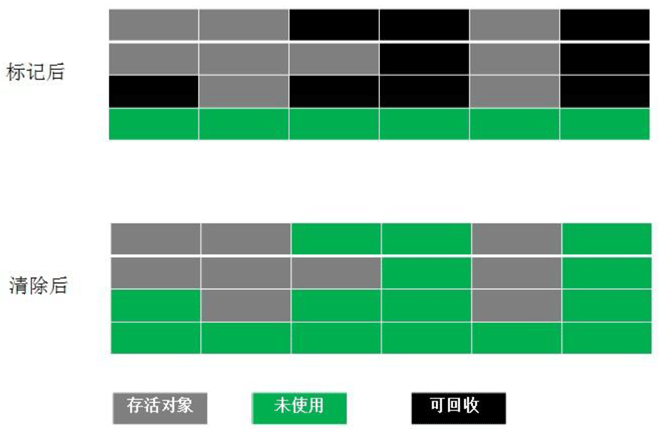
\includegraphics[width=0.7\linewidth]{figures/sign_remove.png}
		      \caption{signremove}
		      \label{fig:sign_remove}
	      \end{figure}
	\item 标记整理: 标记完毕之后, 让所有存活的对象向一端移动
	\item 复制算法: 分别8:1的Eden去和survivor区
	      \begin{figure}
		      \centering
		      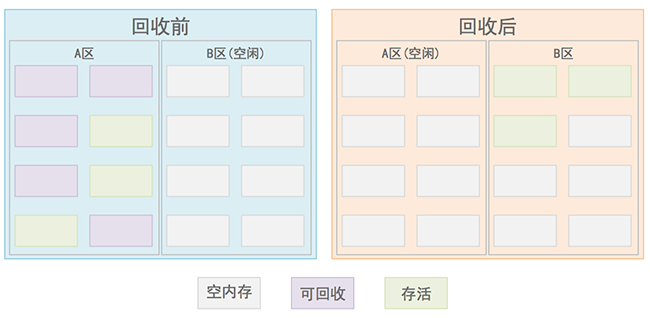
\includegraphics[width=0.7\linewidth]{figures/jvm_copy.jpg}
		      \caption{jvmcopy}
		      \label{fig:jvm_copy}
	      \end{figure}
	\item 分代收集算法-重点 \par
	      一般将Java分成新生代和老年代, 新生代使用复制算法, 老年代使用标记整理算法.
\end{enumerate}
\subsubsection{JVM的主要组成部分及其作用?}
JVM包含两个子系统和两个组件, 两个子系统为Class loader(类加载), Execution engin(执行引擎); 两个组件为 Runtime data area(运行时数据区), native Interface(本地接口)

\begin{enumerate}
	\item Class loader: 根据给定的额全限定类名(如:java.lang.object)来装在class文件到Runtime data area中的method area.
	\item Execution engine(执行引擎): 执行classes中的指令
	\item native Interface(本地接口): 与native libraries交互, 是其他编程语言交互的接口.
	\item Runtime data area(运行时数据区): 这就是我们常说的jvm的内存
\end{enumerate}
\par
\textbf{作用:} 首先通过编译器吧java代码转换成字节码, 类加载器(ClassLoader) 再把字节码加载到内存中, 将其放在运行时数据区(Runtime data area)的方发区内, 而字节码文件知识jvm的一套指令集规范, 并不能直接交给底层操作系统去执行, 因此需要特定的命令解析器执行引擎(Execution Engine), 将字节码翻译成底层系统指令, 在交由CPU去执行, 而这个过程中需要调用其他语言的本地库接口(Native Interface) 来实现整个程序的功能.
\par
Java程序运行机制步骤
\begin{enumerate}
	\item 编码: IDEA等IDE进行编码java, 后缀.java
	\item 编译: javac 将源代码编译成字节码文件,字节码文件的后缀名为.class
\end{enumerate}
类的加载是将类的.class文件中的二进制数据读入到内存中, 将其放在运行时数据区的方法去内, 然后在堆区创建一个java.lang.Class对象, 用来封装类在方区内的数据结构.
\subsubsection{JVM运行时数据区}
运行时数据区由如下几个区域构成
\begin{enumerate}
	\item 程序计数器(PC): 当前线程所执行字节码的行号指示器, 字节码解析器的工作是通过改变这个计数器的值, 来选去下一条需要执行的字节码指令.
	\item java虚拟机栈(Java Virtual Machine Stacks): 用于存储局部变量表, 操作数栈, 动态链接, 方法出口等信息.
	\item 本地方法栈(Native Method Stack) : 与虚拟机栈的作用是一样的, 只不过虚拟机栈是服务Java方法的, 而本地方法栈是为虚拟机调用Native方法服务的.
	\item Java堆(Java Heap): Java 虚拟机中内存最大的一块, 是被所有线程共享的, 几乎所有的对象实例, 都在这里分配内存;
	\item 方法区(Method Area): 用于存储已被虚拟机加载的类信息, 常量, 静态变量, 及时编译后的代码等数据.
\end{enumerate}
\begin{figure}
	\centering
	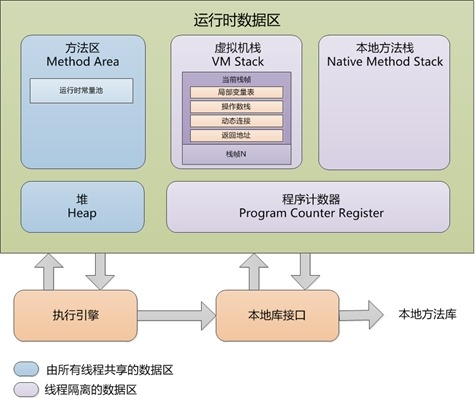
\includegraphics[width=0.7\linewidth]{figures/jvm.jpg}
	\caption{jvm}
	\label{fig:jvm}
\end{figure}
\subsubsection{JVM运行时数据区这些方法的关系}
\begin{figure}
	\centering
	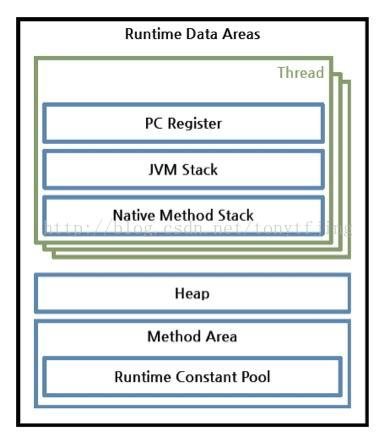
\includegraphics[width=0.7\linewidth]{figures/jvmRunTime.jpg}
	\caption{jvmRunTime}
	\label{fig:jvmRunTime}
\end{figure}
可以看到PC指针和虚拟机栈和本地方法栈是线程独有的. 而堆,方法区和运行时常量池是属于线程共享
\subsubsection{永久代PermGen 和 元空间Metaspace 区别}
\begin{enumerate}
	\item 永久代PermGen : 是jdk1.7 对于方发区的实现. 由于动态生成类的情况比较容易出现永久代的内存溢出, 抛出异常. 而且字符串存储在永久代中容易出现性能问题和内存溢出.
	\item 元空间MetaSpace: 存在于本地内存.
\end{enumerate}
\subsubsection{说一下堆栈的区别?}
\textbf{物理地址}
\par
堆的物理地址分配对对象是不连续的. 因此, 性能慢些. 在GC的时候也要考虑到不连续的分配, 所以后各种算法. 比如, 标记-清除, 复制, 标记压缩, 分代(即新生代生活复制算法, 老年代使用标记压缩算法);
\par
栈使用的是数据结构中的栈, 先进后出的原则, 物理地址分配是连续的. 所以性能快.
\par
\textbf{内存区别}
\par
堆因为是不连续的, 所以分配的内存是在\textbf{运行期}确认的, 因此大小不固定. 一般堆大小远大于栈.
\par
栈是连续的, 所以分配的内存大小要在编译器就确认, 大小是固定的.
\par
\textbf{程序的可见度}
\par
堆对于整个应用程序都是共享, 可见的.
栈只对于线程是可见的. 所以也是线程私有. 他的生命周期和线程相同.
TIPS:
\begin{enumerate}
	\item 静态变量放在方法区.
	\item 静态的对象还是放在堆.
\end{enumerate}


\subsubsection{常见的垃圾收集器?}
(1) Serial收集器, 单线程收集器, 会stop the word. \par
\begin{figure}
	\centering
	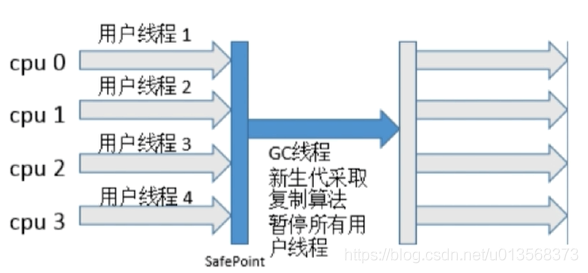
\includegraphics[width=0.7\linewidth]{figures/Serial.png}
	\caption{Serial}
	\label{fig:Serial}
\end{figure}
(2) ParNew(Parallel Old)收集器, 是Serial收集器的多线程版本. 然后, 并行收集垃圾工作, 此时用户线程也是停止的状态 \par
\begin{figure}
	\centering
	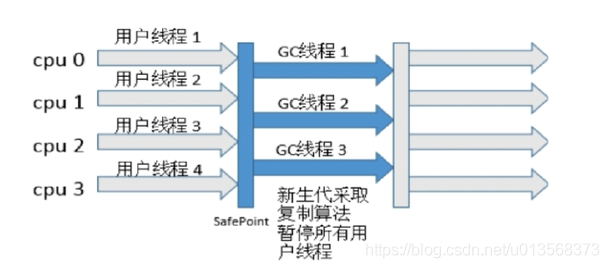
\includegraphics[width=0.7\linewidth]{figures/ParNew.png}
	\caption{ParNew}
	\label{fig:ParNew}
\end{figure}
(3) Parallel Scavenge 收集器(新生代) \par
多线程收集器, 同样是针对新生代. 停顿时间较短 \par
\begin{figure}
	\centering
	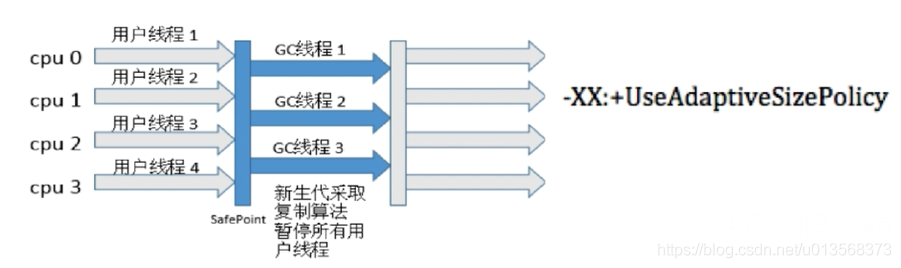
\includegraphics[width=0.7\linewidth]{figures/parallelscavenge.png}
	\caption{parallelscavenge}
	\label{fig:parallelscavenge}
\end{figure}
(4) Serial Old 收集器(老年代) \par
使用标记整理算法收集老年代垃圾, 单线程. \par
(5) Parallel old 收集器(老年代) \par
标记整理算法, 多线程 \par
(6) CMS收集器 \par
简单来说, 在垃圾回收线程几乎能做到与用户线程同时工作, 使用标记清除算法.
\begin{figure}
	\centering
	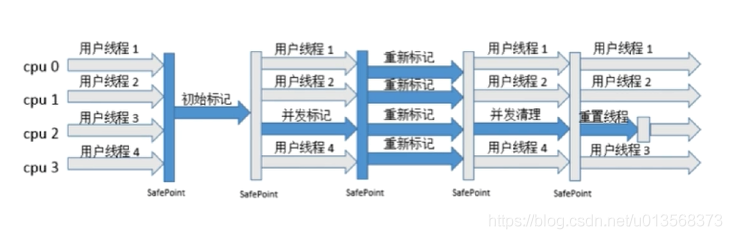
\includegraphics[width=0.7\linewidth]{figures/cms.png}
	\caption{cms}
	\label{fig:cms}
\end{figure}
(7) G1 收集器 \par
使用复制 + 标记 - 整理算法 收集新生代和老年代垃圾.
\subsubsection{内存分配与回收策略. }
1. MinorGC 和 Full GC 有什么不同? \par
MINORGC: 新生代垃圾回收, 回收速度一般较快 \par
MajorGC: 老年代GC, 回收速度较慢 \par
FULLGC: 重GC, 会清理整个空间包括年轻代和老年代. \par
2. 什么时候对象进入老年代 \par
(1) 大对象直接进入老年代 \par
(2) 空间分配担保: 当TO被填满后 当其中的对象还村或者, 剩下的对象直接存入老年代 \par
(3) 年龄判定: 如果Survivor空间中相同年龄多有对象大小的总和大于Survivor空间的一半, 年龄大于或等于改年龄的对象就可以直接进入老年代, 如需达到要求的年龄 \par
\subsubsection{虚拟机性能监控和故障处理工具}
jvisualvm 可视化监控.
\subsubsection{简述JVM中类加载机制}
类加载过程: 加载, 验证, 准备, 解析和初始化. \par
(1) 加载 \par
1. 通过类的全限定名获取此类的二进制字节流 \par
2. 将这个字节流所代表的的静态存储结构转化为方发区的运行时数据结构 \par
3. 在内存中生成一个代表这个类的java.lang.Class对象, 作为方发渠这个类的各种数据的访问入口 \par
(2) 验证 \par
为了却表Class文件的字节流中包含的信息符合当前的虚拟机的要求, 并且不会危害虚拟机自身的安全. \par
(3) 准备 \par
正式为类变量(static修饰的)分配内存并设置类变量初始值的节点, 这些变量所使用的的内存都将在\textbf{方法区}中进行分配 \par
(4) 解析 \par
虚拟机将常量池内的符号引用替换为直接引用的过程. 主要对类过接口, 字段, 类方法, 接口方法的解析, 主要是静态链接, 方法主要是静态方法和私有方法. \par
\subsubsection{对象的访问定位?}
目前主流的访问方式有句柄和直接指针两种方式.

\begin{enumerate}
	\item 指针: 指向对象, 代表一个对象再内存中的起始地址
	\item 句柄: 可以理解为指向指针的指针, 维护者对象的地址. 句柄不直接指向对象, 而是指向对象的地址(句柄不发生变化, 指向固定内存你地址), 再由对象的指针指向对象的真实内存地址.
\end{enumerate}
\textbf{句柄访问}
\par
Java堆中划分出一块内存作为句柄池, 引用中存储对象的句柄地址, 而句柄中包含了\textbf{对象实例数据}与\textbf{对象类型数据}各自的决堤地址信息, 具体构造如下图所示:
\begin{figure}
	\centering
	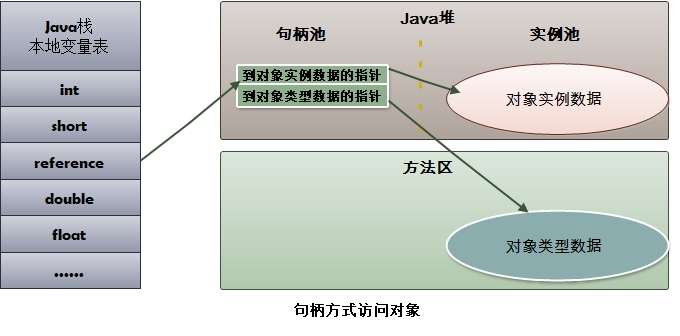
\includegraphics[width=0.7\linewidth]{figures/jvm_handler.jpg}
	\caption{jvmhandler}
	\label{fig:jvm_handler}
\end{figure}
\textbf{直接指针}
\par
\begin{figure}
	\centering
	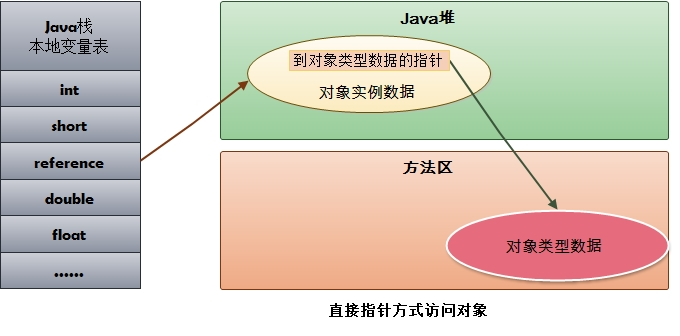
\includegraphics[width=0.7\linewidth]{figures/jvm_point.jpg}
	\caption{jvmpoint}
	\label{fig:jvm_point}
\end{figure}
\subsubsection{垃圾回收器的基本原理是什么?}
\textbf{可达性分析}
\par
GC采用有向图的方式记录和管理堆中的所有对象. 通过这种方式确定哪些对象是"可达的", 哪些对象是"不可达的", 当GC确定一些对象为"不可达"时, GC就有责任回收这些内存空间.
程序员可以手动执行System.gc(), 通知GC运行, 但是Java语言规范并不保证GC一定会执行.
\par
\textbf{引用计数法}
为每个对象创建一个引用技术, 有对象引用时计数器+1, 引用被释放是技术-1, 当计数器为0时就可以被回收. 优缺点, 不能解决循环引用的问题.
\subsubsection{在java中, 对象什么时候可以被垃圾回收?}
当对象变的不可触及的时候, 这个对象就可以被回收了, 垃圾回收不会发生在永久代, 如果永久代满了或者是超过了临界值, 会触发完全垃圾回收(full gc), 会导致Stop-the-world.
\subsubsection{如何判断对象已经死亡?}
(1) 引用计数法, 标记为零. 缺点难以解决互相引用问题 \par
(2) 可达性分析, 当一个对象到GC Root对象没有任何路径可达. \par
(3) 上面两种都是暂时处于缓刑阶段, 真正宣告一个对象死亡, 至少要经历两次标记过程.
\subsubsection{简述强, 软, 弱, 虚引用?}
(1) 强引用 \par
如果一个对象具有强引用, 垃圾回收期绝不会回收它 \par
(2) 软引用(SoftRef) \par
如果内存足够, 垃圾回收期就不会回收塔, 如果内存不足了, 就会回收这些对象的内存. 可以实现内存敏感的告诉缓存. \par
(3) 弱引用(WeakRef) \par
弱引用关联的对象只能生存到下一次垃圾回收之前. \par
(4) 虚引用(ReferenceQue) \par
如果一个对象仅持有虚引用, 那么他就和没有任何引用一样, 在任何时候都可能被垃圾回收. 必须和引用队列一起联合使用.\par
\textbf{区别:} \par
软弱引用都是发生在垃圾回收动作之后, 虚引用发生在垃圾回收动作之前.